
%==============  N E W  ==== C H A P T E R ==============%
\chapter{Vorbereitung f�r Vergleich}
\label{chapter:Vorbereitung}
\index{Vorbereitung f�r Suche|(}
Bevor ein Vergleich zwischen den verschiedenen Search-Engines gemacht werden kann, sollte ein �berblick �ber die Search-Engines erstellt werden.

%==============  N E W  ==== S E C T I O N ==============%
\section{Windows Index Suche}
\label{sec:WindowsSearchEngine}

Standardm�ssig werden bei Windows nur einzelne Ordner indiziert. Gleichzeitig indiziert Windows nicht die kompletten Datei Inhalte, sondern lediglich die Einstellungen und deren Metadaten.\\
Um die Inhalte auch zu indizieren, muss dies in den Einstellungen ge�ndert werden (siehe Abbildung \ref{fig:WindowsSearchDefault} rechte Seite).

Um nun ein Netzlaufwerk indexieren zu k�nnen (was hier auch gew�nscht ist), muss ein Add-in von Microsoft installiert werden. Dieses nennt sich \flqq Windows Desktop Search: Add-in for Files on Microsoft Networks\frqq\ und ist auf der Microsoft Homepage verf�gbar\footnote{\url{http://www.microsoft.com/en-us/download/details.aspx?id=3383}}.

Da dies leider nach einem Neustart nicht funktionierte, wurde eine weitere M�glichkeit gesucht.\\
So wurde gem�ss dem Microsoft Technet-Artikel\footnote{\url{http://social.technet.microsoft.com/Forums/windows/en-US/afb904c1-1c61-4aae-b6b1-5cf525b9f8de/how-do-i-get-windows-7-to-index-a-network-mapped-drive?forum=w7itpronetworking}} folgende Punkte erledigt:

 \begin{itemize}
\item  Erstellen einer neuen Windows Library \flqq ZHAW Docs\frqq  \ erstellt.
\item Erstellen eines neuen Ordners C:\textbackslash ZHAW Docs
\item Hinzuf�gen des neu erstellten Ordners zur neuen Library
\item Ordner C:\textbackslash ZHAW Docs l�schen
\item �ber cmd (als Administrator) folgenden Befehl ausf�hren:\\
mklink /d \grqq C:\textbackslash ZHAW Docs\grqq \  \grqq \textbackslash \textbackslash<IP Synology>\textbackslash <Share-Path>\grqq \\
Mit diesem Befehl wurde ein symbolischer Link des Netzwerkpfades auf den lokalen Pfad gesetzt.

\end{itemize}

\newpage
\begin{figure}[h!]
\centering
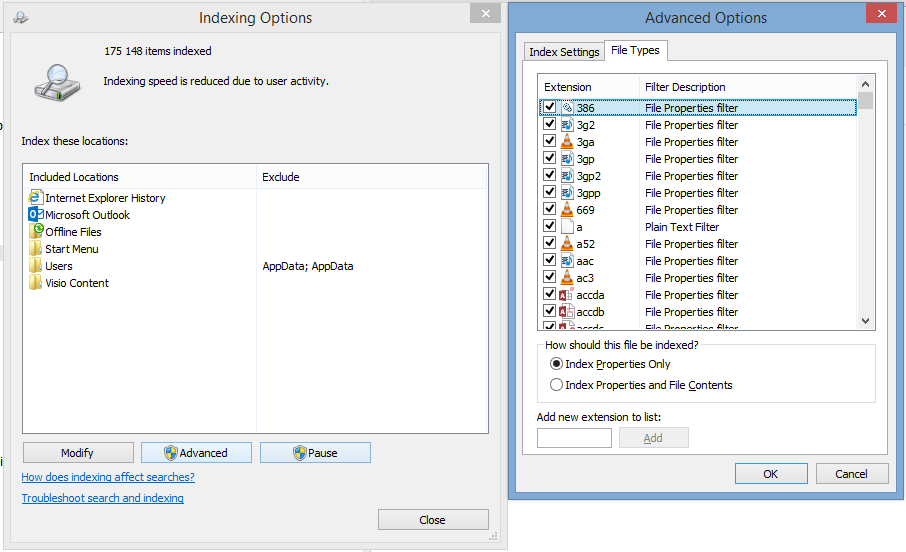
\includegraphics[width=0.95\textwidth]{WindowsSearchDefault.PNG} 
\caption[Windows Indexing - Default Einstellungen]{Windows Indexing - Default Einstellungen\\Quelle: eigener Screenshot}
\label{fig:WindowsSearchDefault}
\end{figure}

Da die Indizierung �ber den Softlink gem�ss Anleitung leider nicht wie gew�sncht funktionierte, wurden alle Schuldaten auf dem Windows Rechner auf die lokale Festplatte kopiert und indiziert. So kann sichergestellt werden, dass ein fairer Vergleich der Resultate stattfinden kann.


%==============  N E W  ==== S E C T I O N ==============%
\newpage
\index{Lucene Syntax|see{Syntax Lucene}}
\index{Syntax Lucene|(}
\section{Syntax f�r Suche mit Lucene / Luke}
\label{sec:LukeQuery}

\begin{figure}[h!]
\centering
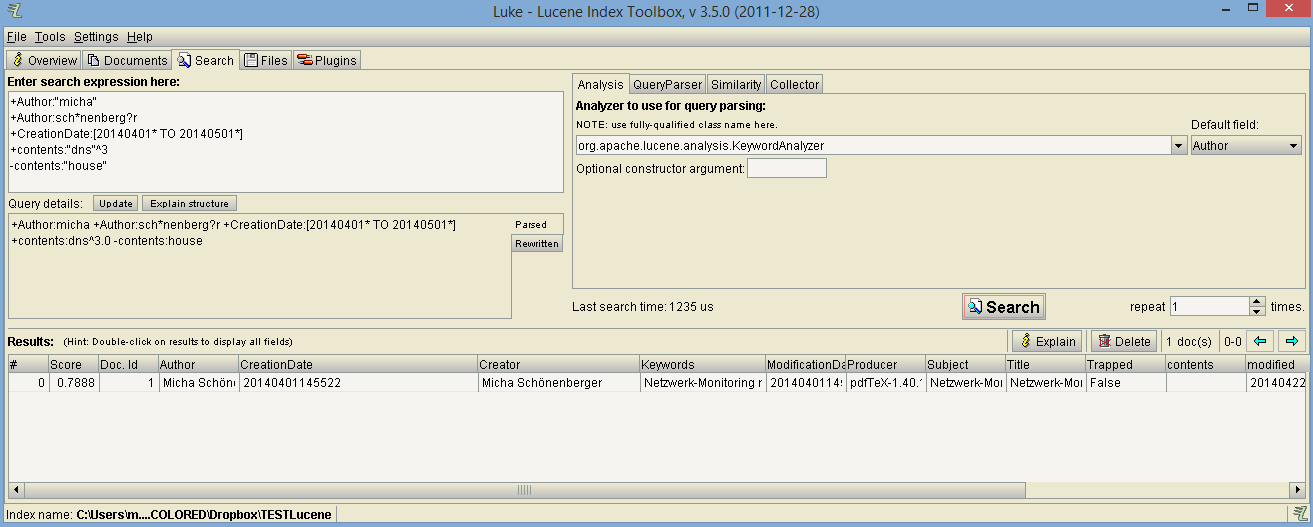
\includegraphics[width=1\textwidth]{Luke-Query.PNG} 
\caption[Such-Maske von Luke]{Such-Maske von Luke\\ Quelle: eigener Screenshot}
\label{fig:Luke-Query}
\end{figure}

Anbei einige Beispiele, wie man den Syntax optimal einsetzen kann f�r sie Suche mit Luke/Lucene:
%==============  N E W  ==== S U B - S E C T I O N ==============%
\subsection{Felder}
\begin{tabularx}{\columnwidth}{|l|X|} \hline
contents:prtg & sucht das Wort \flqq prtg\frqq\ im Feld contents   \\ \cline{1-2}
Author:micha monitor & sucht das Wort \flqq micha\frqq\ im Feld Author, \\ 
 & das Wort \flqq netzwerk\frqq\ im default Feld \\ \cline{1-2}
contents: \grqq mit prtg\grqq \  & sucht die W�rter \flqq mit prtg\frqq\ als Ganzes im Feld contents \\   \cline{1-2}
\end{tabularx}
%==============  N E W  ==== S U B - S E C T I O N ==============%
\subsection{Wildcard Suche}
\begin{tabularx}{\columnwidth}{|l|X|} \hline
pr?g	& Das ? ersetzt einen einzelnen Charakter. So wird hier \\
 & z.B. nach \flqq prtg\frqq, aber auch nach \flqq prag\frqq \  gesucht \\ \cline{1-2}
bildschirm* & * steht f�r beliebig viele Zeichen (0 bis x) .\\
& Suche nach z.B. \flqq bildschirmeingabe\frqq\ oder \flqq bildschirme\frqq\\ \cline{1-2}
ver*en & * steht auch hier f�r beliebige Zeichen (0 bis x)\\
& Suche nach z.B. \flqq verwerfen\frqq\, \flqq verwalten\frqq\  oder \flqq veruntreuen\frqq \\ \cline{1-2}
\end{tabularx}
 
Grunds�tzlich gilt: * und ? d�rfen nicht am Anfang einer Suchanfrage stehen.\\
Anmerkung: Bei Luke gibt es jeodch eine Einstellung, mit der * am Anfang erlauben sein darf.
%==============  N E W  ==== S U B - S E C T I O N ==============%
\subsection{Fuzzy Suche}
Die Fuzzy Suche basiert auf dem Levenshtein Distanz Algorithmus\footnote{siehe \url{http://www.levenshtein.de/}}, auf welchen hier nicht eingegangen wird.\\
Um eine Fuzzy Suche durchzuf�hren, wird mit der Tilde ($\sim$) gearbeitet.

\begin{tabularx}{\columnwidth}{|l|X|} \hline
roam$\sim$ & Sucht �hnliche W�rter zu roam \\ \cline{1-2}
roam$\sim$0.8 & Gibt die gesuchte �hnlichkeit an [0-1]. Je gr�sser die Zahl, desto �hnlicher. \\ \cline{1-2}
\end{tabularx}

%==============  N E W  ==== S U B - S E C T I O N ==============%
\subsection{Proximity Suche (Nachbarschaftliche)}
Lucene erlaubt es, zwei W�rter in einer bestimmten Distanz zu suchen.

\begin{tabular}[t]{|l|l|} \hline
 \multirow{2}{5.75cm}{\grqq prtg monitor\grqq $\sim$10} & Sucht die W�rter \flqq prtg\frqq \ und \flqq monitor\frqq\ mit einem \\
 & maximalen Abstand von 10 W�rtern.\\  \cline{1-2}

\end{tabular}
%==============  N E W  ==== S U B - S E C T I O N ==============%
\subsection{Range Suche (Bereichssuche)}
Lucene erlaubt es, zum Beispiel Daten in einem bestimmten Bereich zu suchen.

\begin{tabular}[t]{|l|l|} \hline
 \multirow{2}{5.75cm}{modified:[20140501 TO 20140515]}&  Sucht eine Datei mit einem �nderungsdatum \\
 & zwischen dem \flqq 01.05.2014\frqq\ und \flqq 15.05.2014\frqq\\ \cline{1-2}
 
  \multirow{2}{5.75cm}{Title:\{Anton TO Max\}}&  Sucht eine Datei mit dem Titel \\
 & zwischen \flqq Anton\frqq\ und \flqq Max\frqq\ (alphabetisch)\\ \cline{1-2}
 \end{tabular}

%==============  N E W  ==== S U B - S E C T I O N ==============%
\subsection{Boosting Suche (verst�rktes Suchen)}
\label{subsec:Boosting}
Lucene erlaubt es, gewissen Suchbegriffen eine st�rkere Gewichtung zu verleihen. Durch diesen Boost wird das Ergebnis die Relevanz der gefundenen Dateien ver�ndert.

\begin{tabular}[t]{|l|l|} \hline
 \multirow{2}{5.75cm}{prtg\^\ 4 monitoring}&  Sucht eine Datei mit \flqq prtg\frqq \ und \flqq monitoring\frqq \\
 & wobei \flqq prtg\frqq \ 4-fach gewertet wird.\\ \cline{1-2}
  \end{tabular}


%==============  N E W  ==== S U B - S E C T I O N ==============%
\subsection{Boolsches Suchen}
Ganz wichtig beim Suchen sind die verschiedenen Verkn�pfungen der eingegebenen Suchbegriffe. Erlaubt sind AND, +, NOT, -

\begin{tabular}[t]{|l|l|} \hline

prtg OR monitor & Sucht entweder nach \flqq prtg\frqq \ oder nach \flqq monitor\frqq \\  \cline{1-2}
 \multirow{2}{4cm}{prtg AND monitor} & Sucht nach  \flqq prtg\frqq \ und nach \flqq monitor\frqq . Beide\\
 & W�rter m�ssen im selben Dokument enthalten sein.\\  \cline{1-2}
 
  \multirow{2}{4cm}{prtg NOT monitor} & Sucht ein Dokument, in welchem \flqq prtg\frqq \ vorkommt, \\
   & \flqq monitor\frqq \ aber nicht.\\ \cline{1-2}
  \multirow{2}{4cm}{NOT prtg} & NOT darf nicht mit nur einem Wort verwendet werden.\\
  & Das Resultat wird hier leer sein.\\ \cline{1-2}
  \end{tabular}
  
  
Anstelle von AND kann auch \&\& oder + verwendet werden.\\
Anstelle von NOT kann auch ! oder - verwendet werden.\\

Quelle Kapitel \ref{sec:LukeQuery}: \cite{Luke_Query}
\index{Syntax Lucene|)}







\index{Vorbereitung f�r Suche|)}






